\section{Central Interleaved Boost (Actual Ratings)}

In modern engineering, jumping straight from a conceptual design to physical hardware is a risky and costly approach. Simulation serves as the crucial bridge between theory and reality. By creating a high-fidelity digital twin of a system, designers can validate control logic, analyze transient behaviors, and stress-test components under extreme conditions without the risk of catastrophic hardware failure.

so before doing anything hardware, we must first do simulation of the circuit to fully understand the it and test different faults or errors that we might face.

\subsection{Simulation of Central Boost without MPPT}
R with mosfet asts as a storage system used to mantain voltage of the dc link at 10\,V with hysteresis control
here is the test to see which duty will achieve max power:
\begin{figure}[H]
    \centering
    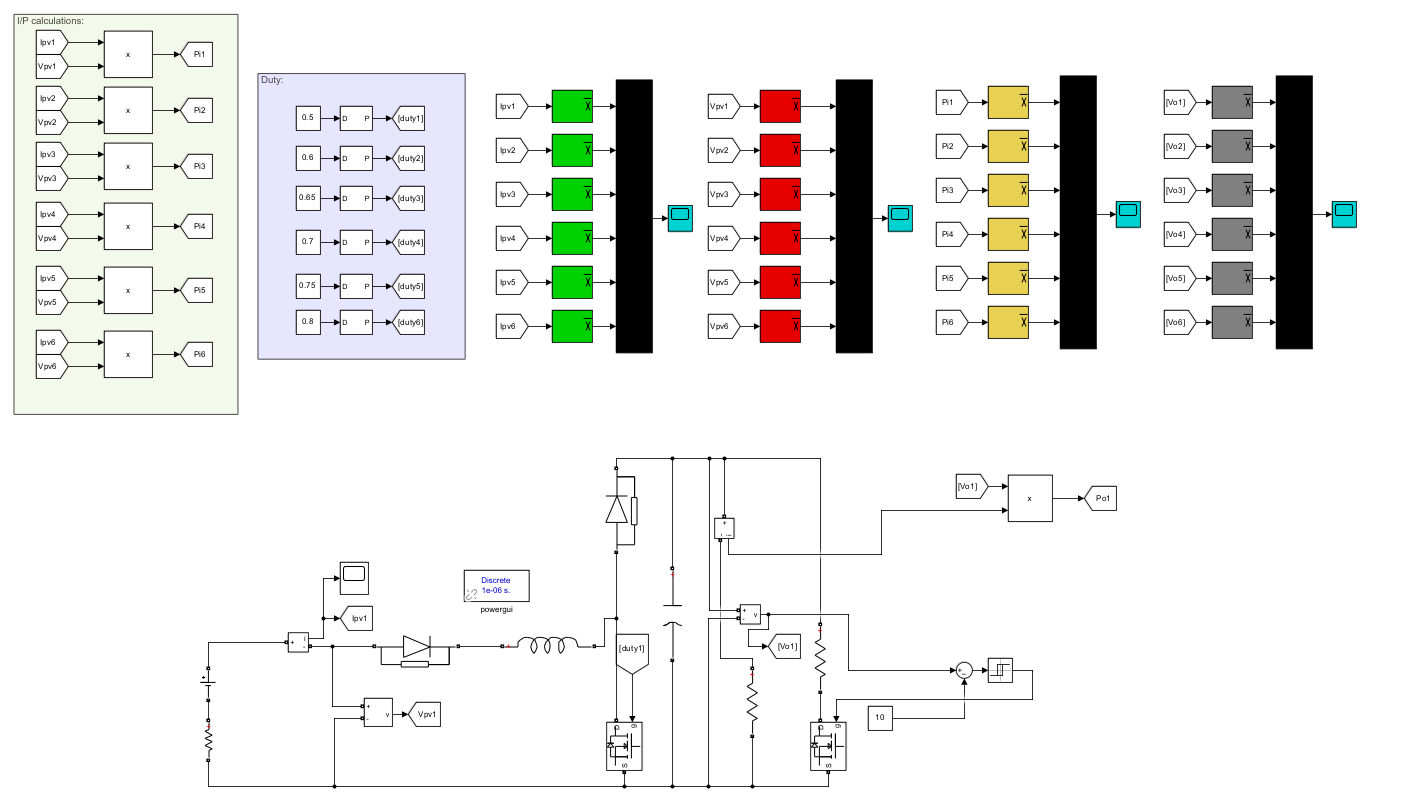
\includegraphics[width=0.85\textwidth]{Figures/5.5.1.png}
    \caption{Central Boost.}
    \label{fig:central boost actual ratings}
\end{figure}

To evaluate the dynamic stability of the system under localized storage integration, the complex photovoltaic (PV) array non-linear characteristic curve is simplified around its operating point utilizing a linear Thevenin equivalent circuit interface. The voltage source and its series internal impedance parameters are defined as:
\begin{itemize}
    \item Thevenin Voltage ($V_{\text{th}}$): $12\text{ V}$
    \item Internal Thevenin Resistance ($R_{\text{th}}$): $6.8\ \Omega$
\end{itemize}

\subsubsection{Hysteresis-Controlled Storage Branch}
A secondary power branch containing a switching MOSFET in series with a storage resistor ($R_{\text{storage}} = 47\ \Omega$) serves as a dynamic energy buffer. This subsystem actively regulates and clamps the output high-voltage DC-link bus at a rigid target command of $V_{\text{DC\_ref}} = 10\text{ V}$. 
\newpage
The regulation is driven by hysteresis control loop tracking the instantaneous DC-link voltage error. The mathematical switching states governing the gate-drive command ($S$) of the storage MOSFET are defined according to the following boundary conditions:

\begin{equation}
    S = 
    \begin{cases} 
      1 & \text{for } V_{\text{DC}} > V_{\text{DC\_ref}} + \Delta H \\
      0 & \text{for } V_{\text{DC}} < V_{\text{DC\_ref}} - \Delta H 
    \end{cases}
\end{equation}

Where $\Delta H$ represents the predefined narrow hysteresis band offset. When the DC-link voltage surpasses the upper boundary threshold, the MOSFET switches to its conduction state ($S=1$), shunting the excess power into $R_{\text{storage}}$ to discharge the bus. Conversely, when the bus voltage drops below the lower band margin, the switch opens ($S=0$) to isolate the storage asset and restore the system voltage envelope across the static load network ($R_{\text{load}} = 100\ \Omega$).

\subsubsection{System Passive Components}
The passive filtering parameters chosen to restrict high-frequency switching ripples within the network are summarized in Table \ref{tab:thevenin_parameters}.

\begin{table}[htbp]
    \centering
    \caption{Thevenin equivalent system and filter parameter metrics.}
    \label{tab:thevenin_parameters}
    \small
    \begin{tabular}{|c|c|c|}
        \hline
        \textbf{Parameter Name} & \textbf{Designation Symbol} & \textbf{Assigned Value} \\ \hline
        Inductance       & $L$                        & $2\text{ mH}$           \\ \hline
        Capacitance      & $C$                        & $2.2\text{ mF}$         \\ \hline
        Storage Resistance      & $R_{\text{storage}}$       & $47\ \Omega$            \\ \hline
        Equivalent Load         & $R_{\text{load}}$          & $100\ \Omega$           \\ \hline
    \end{tabular}
\end{table}

\subsubsection{Results}
\begin{figure}[H]
    \centering
    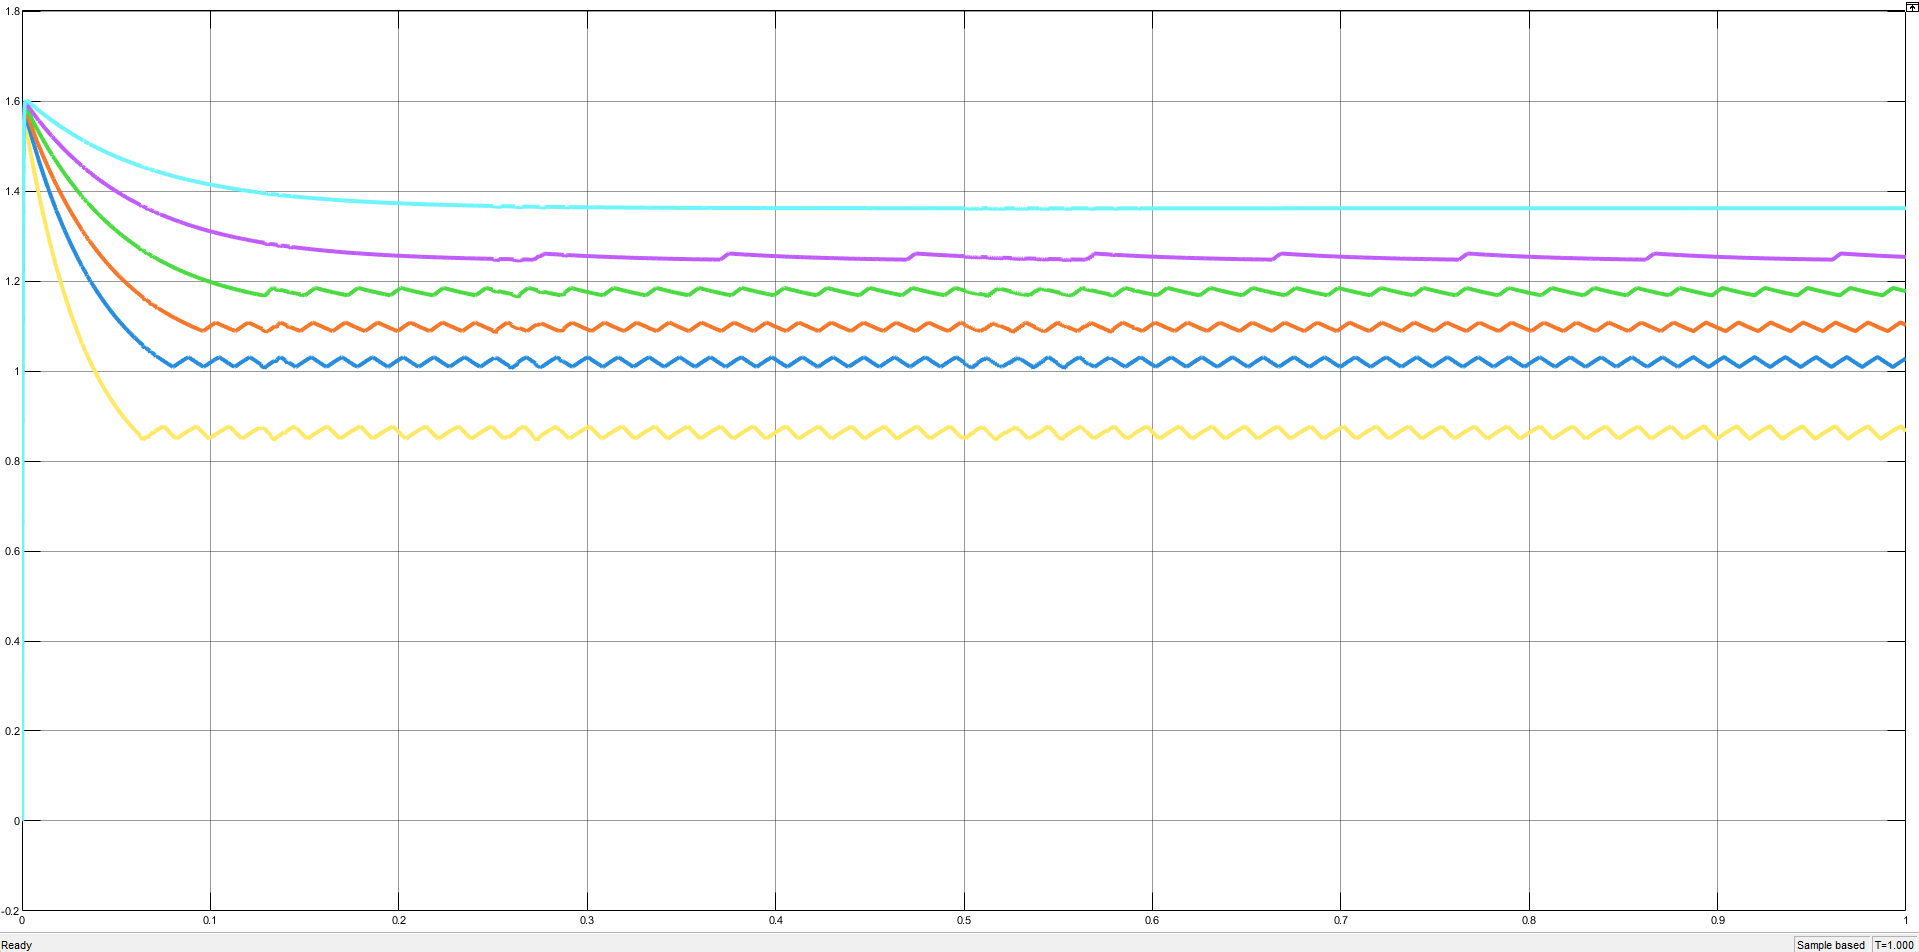
\includegraphics[width=0.9\textwidth]{Figures/5.5.2.png}
    \caption{Input Currents.}
    \label{fig: input current of central interleaved boost actual ratings}
\end{figure}
\begin{figure}[H]
    \centering
    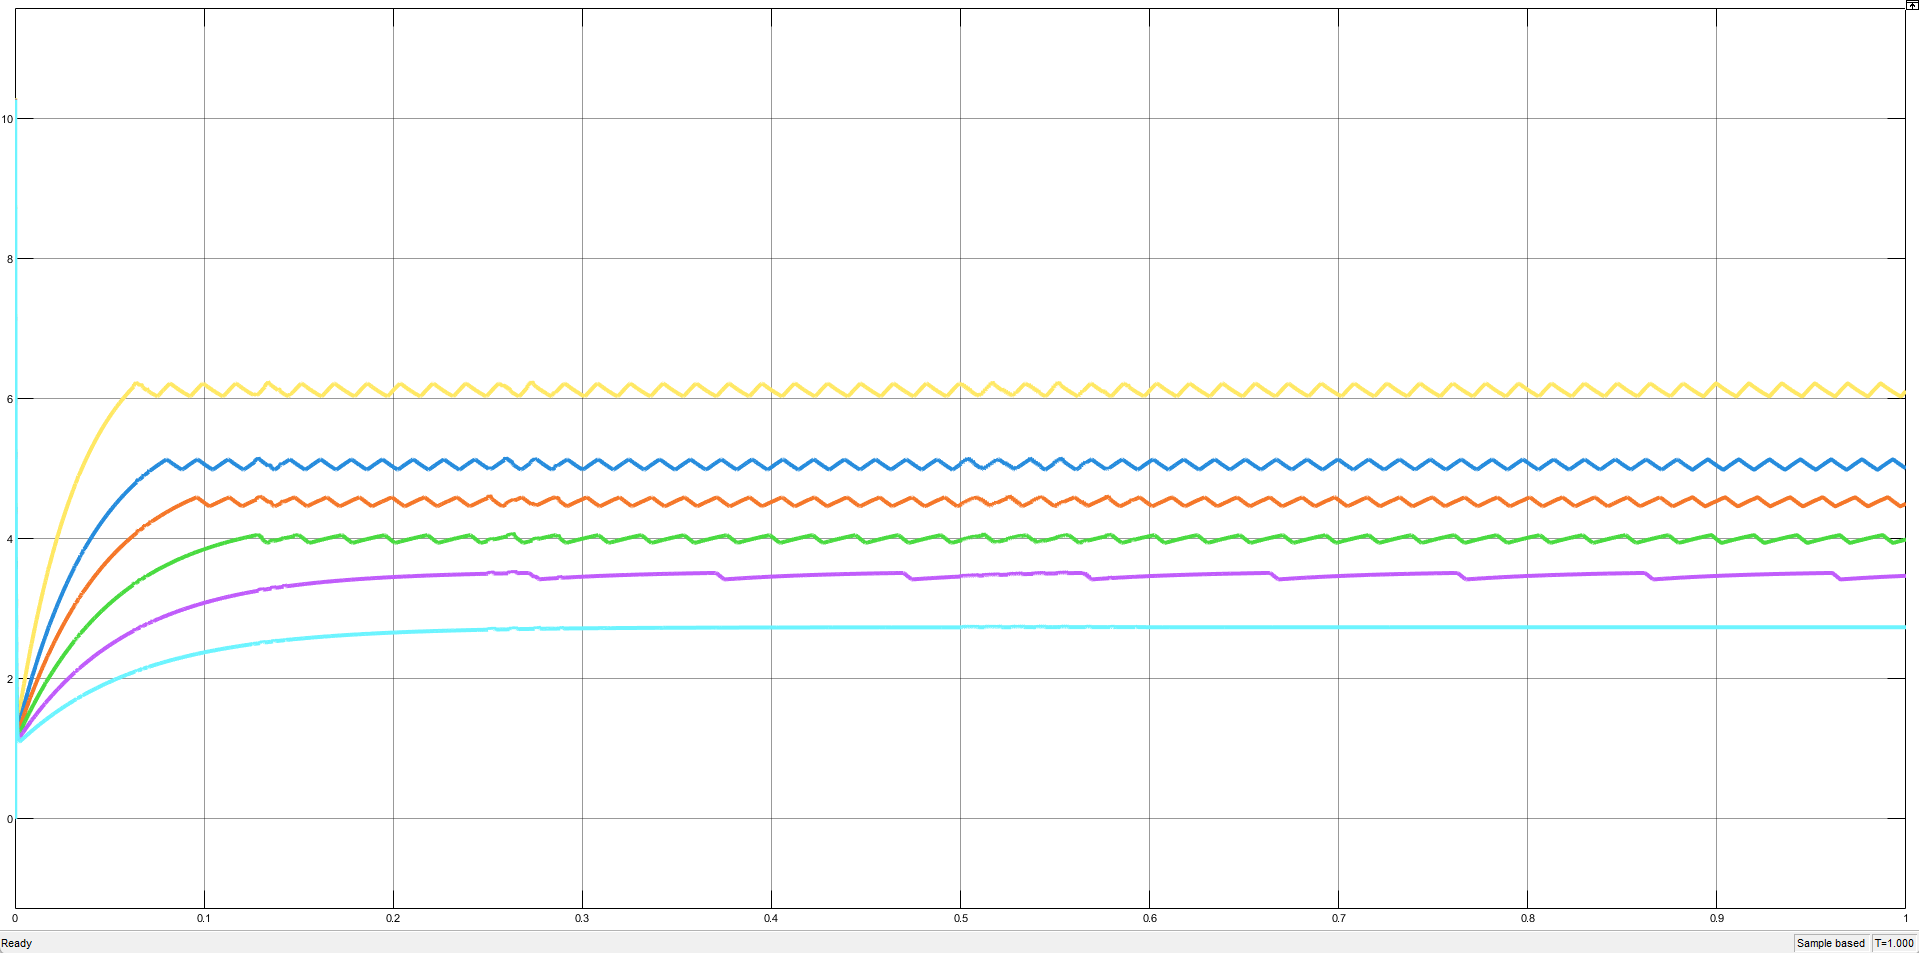
\includegraphics[width=0.9\textwidth]{Figures/5.5.3.png}
    \caption{Input Voltages.}
    \label{fig: input voltages of central interleaved boost actual ratings}
\end{figure}
\begin{figure}[H]
    \centering
    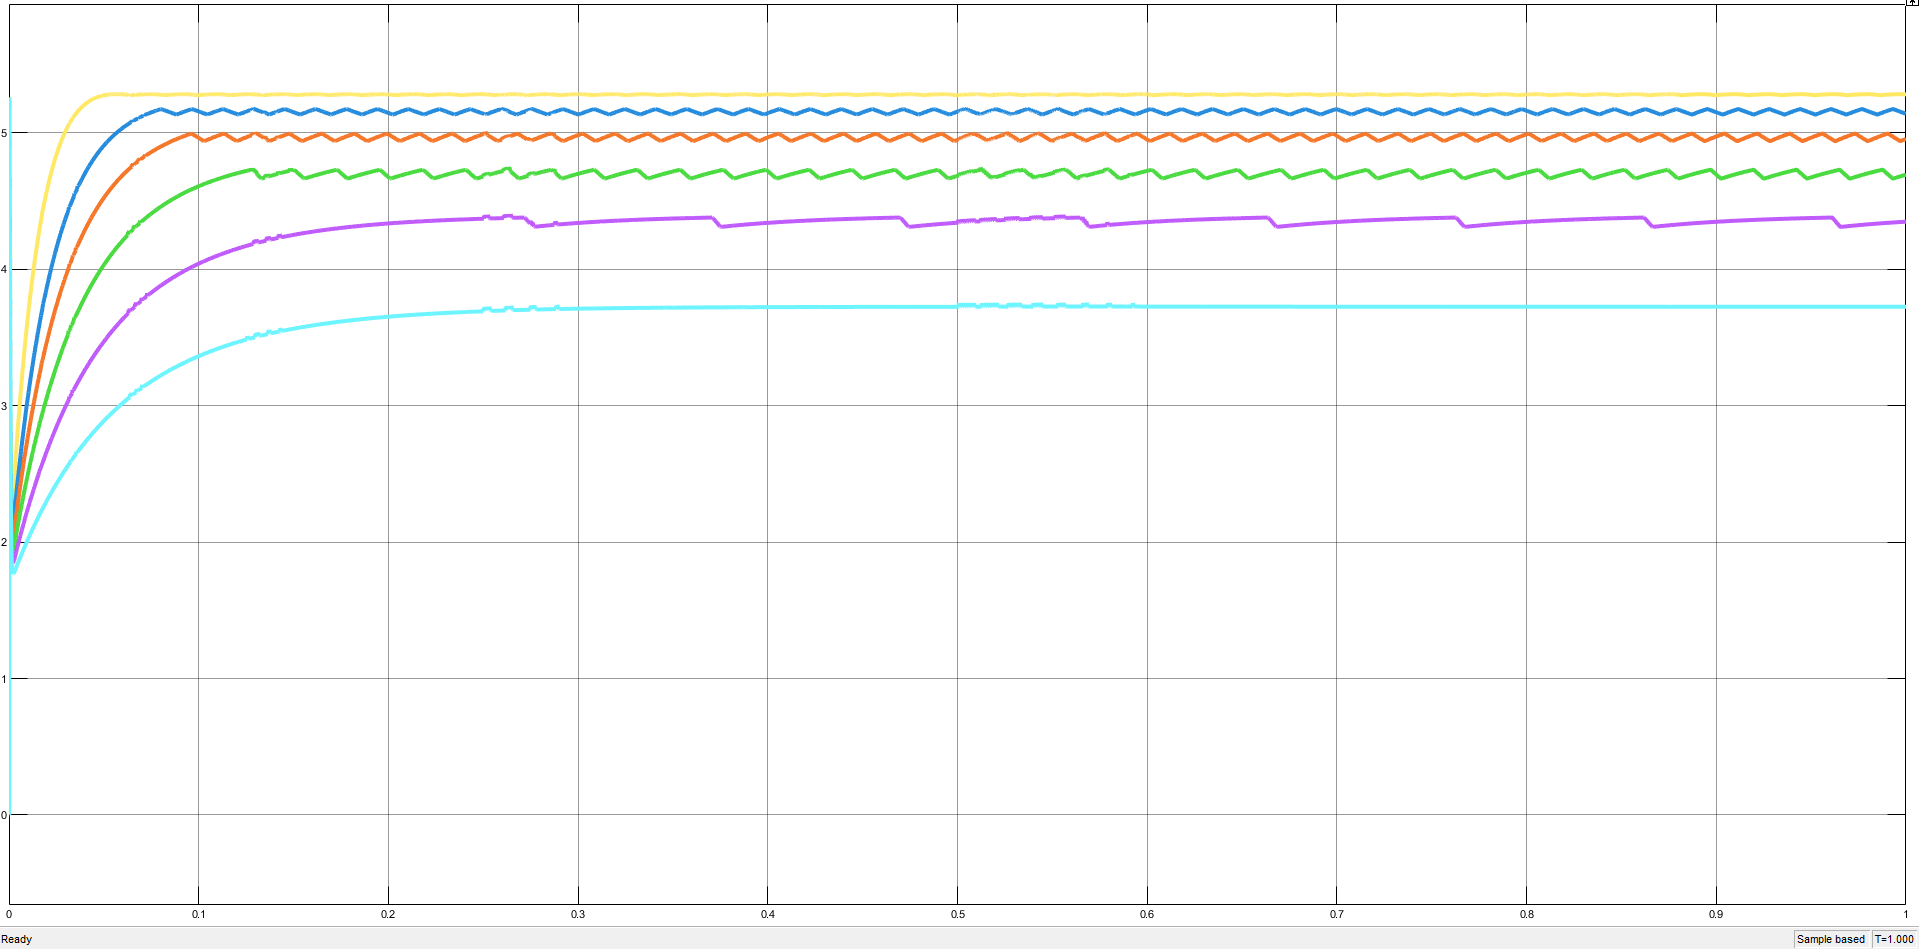
\includegraphics[width=0.9\textwidth]{Figures/5.5.4.png}
    \caption{Input Power.}
    \label{fig: input power of central interleaved boost actual ratings}
\end{figure}
\begin{figure}[H]
    \centering
    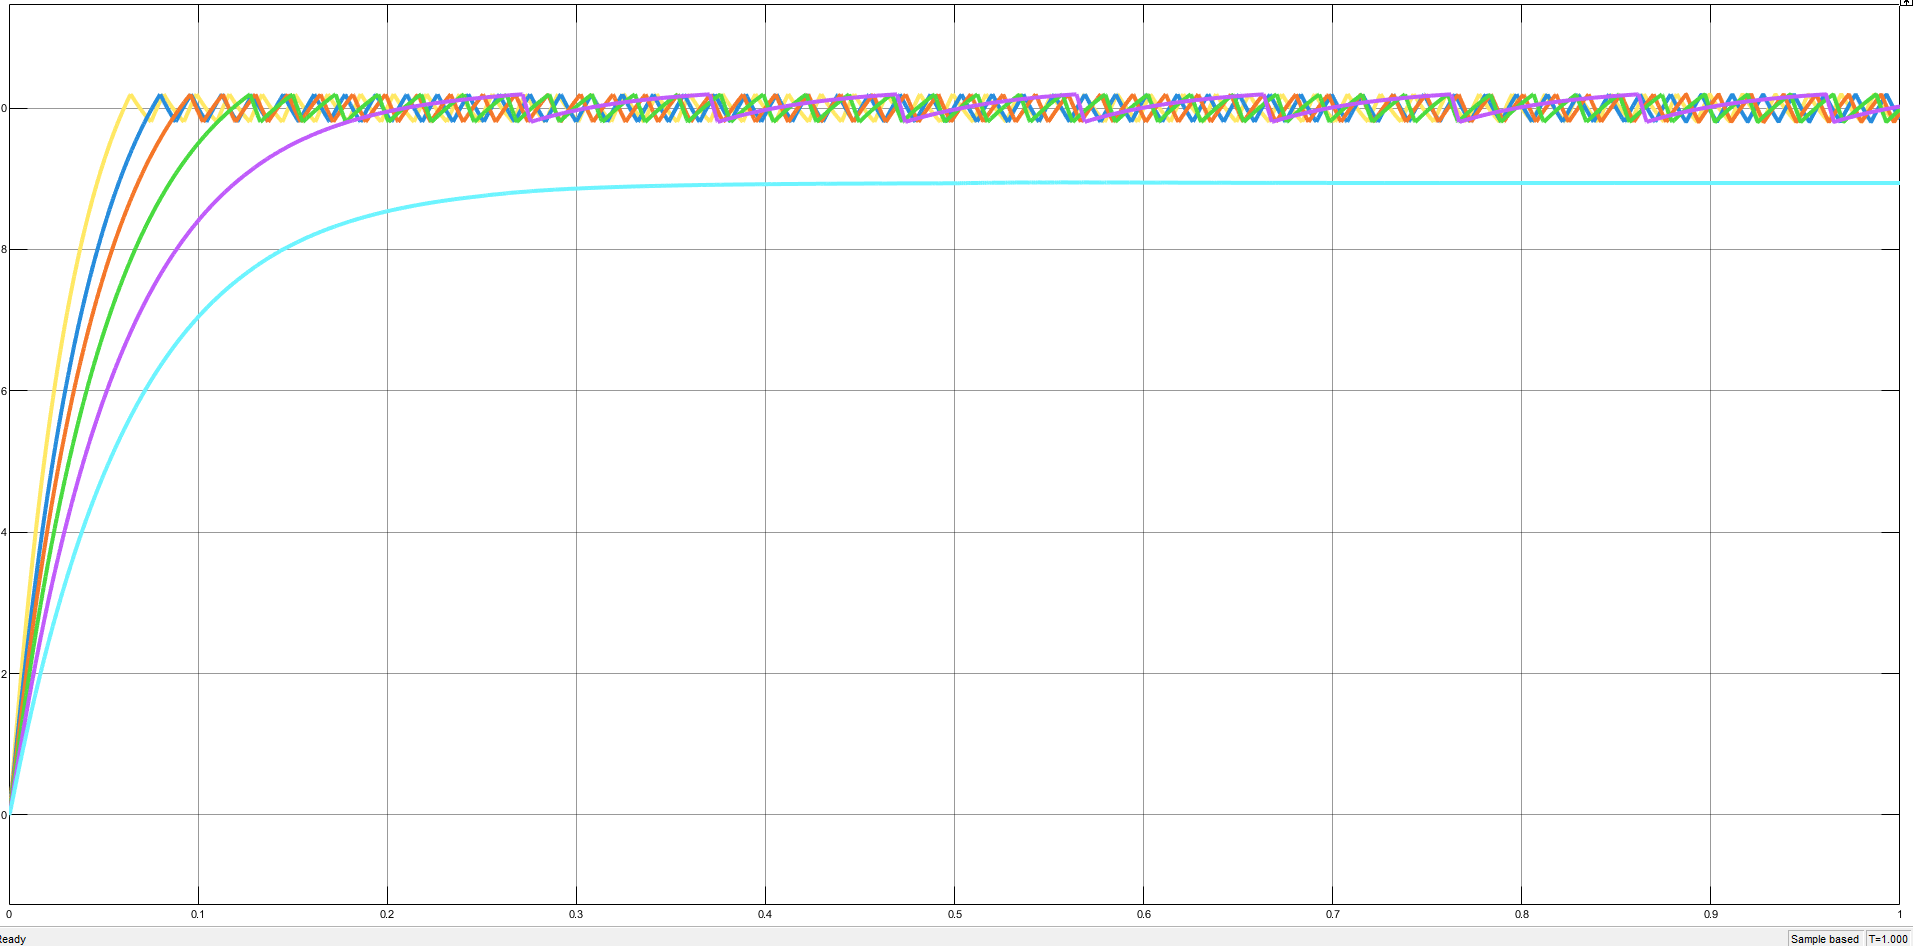
\includegraphics[width=0.9\textwidth]{Figures/5.5.5.png}
    \caption{Output Voltages.}
    \label{fig: output voltages of central interleaved boost actual ratings}
\end{figure}

As shown in the simulation results, the maximum power extraction point occurs precisely at a duty cycle of $D = 0.65$.

\subsection{Simulation of Central Interleaved Boost with MPPT}
\begin{figure}[H]
    \centering
    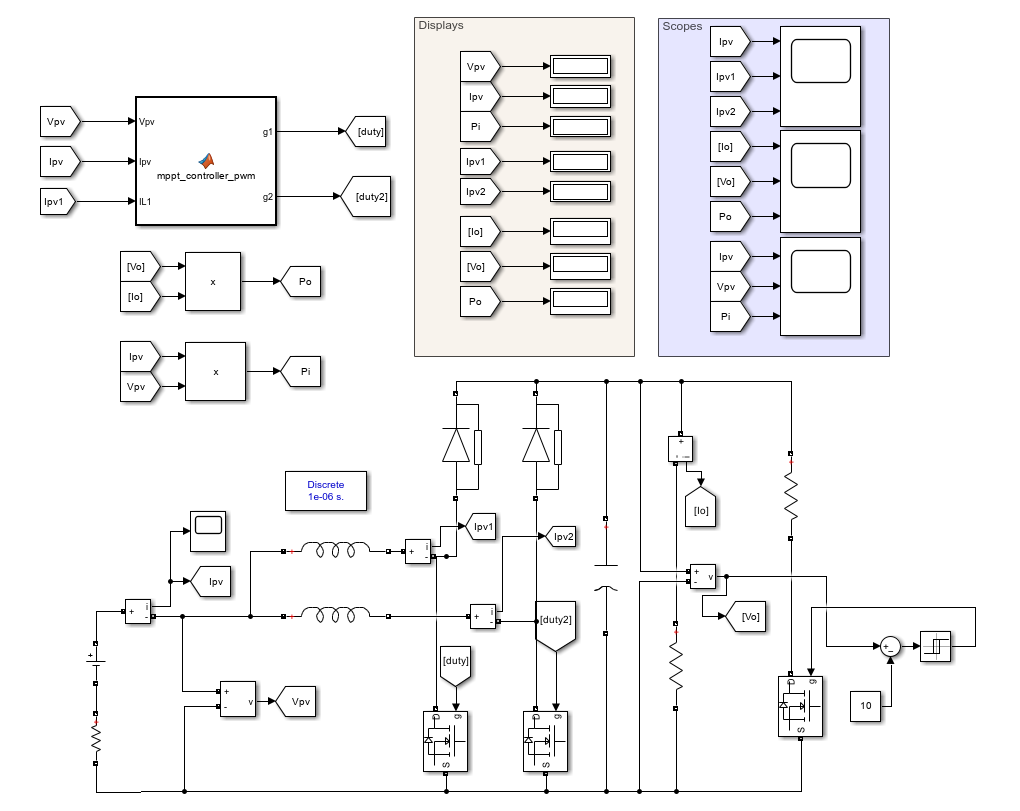
\includegraphics[width=0.9\textwidth]{Figures/5.5.6.png}
    \caption{Central Interleaved Boost.}
    \label{fig:central interleaved boost actual ratings}
\end{figure}

\begin{lstlisting}[language=Matlab, caption={MATLAB code implementing the FSM-based global MPPT control loop.}]
function [g1, g2] = mppt_controller_pwm(Vpv, Ipv, IL1)
    persistent V_target Pmax Vbest mode timer;
    persistent err_int_v err_int_i t;
    
    Ts = 1e-6;      
    fsw = 10e3;     
    Tsw = 1/fsw;
    
    if isempty(V_target)
        V_target = Vpv; 
        Pmax = 0;
        Vbest = Vpv;
        mode = 0;
        timer = 0;
        err_int_v = 0;
        err_int_i = 0;
        t = 0;
    end
    
    % ===== Internal Calculation of IL2 =====
    % Based on the nodal equation: Ipv = IL1 + IL2
    IL2 = Ipv - IL1; 
    
    % ===== MPPT Logic (Scanning) =====
    Ppv = Vpv * Ipv;
    V_ramp_rate = 200; 
    
    switch mode
        case 0 % Initialization
            V_target = Vpv;
            Pmax = 0;
            mode = 1;
            
        case 1 % Scanning Downward
            if Ppv > Pmax
                Pmax = Ppv;
                Vbest = Vpv;
            end
            V_target = V_target - (V_ramp_rate * Ts);
            % Stop scan at 50% of starting voltage
            if V_target <= 0.5 * Vbest 
                mode = 2;
            end
            
        case 2 % Return to Vbest
            V_target = Vbest;
            mode = 3;
            timer = 0;
            
        case 3 % Hold and Dwell
            timer = timer + Ts;
            if timer >= 5 
                mode = 0; % Restart scan
            end
    end
    
    % ===== Outer Loop: Voltage Control (Vpv -> Iref) =====
    err_v = Vpv - V_target; 
    
    Kp_v = 1.5; 
    Ki_v = 80;
    
    err_int_v = err_int_v + err_v * Ts;
    err_int_v = max(min(err_int_v, 0.5), -0.5); 
    
    Iref_total = Kp_v * err_v + Ki_v * err_int_v; 
    Iref_total = max(min(Iref_total, 20), 0); 
    
    % ===== Inner Loop: Current Control (Iref -> Duty) =====
    Iref_phase = 0.5 * Iref_total;
    
    err_i1 = Iref_phase - IL1;
    err_i2 = Iref_phase - IL2;
    
    Kp_i = 5; 
    Ki_i = 100;
    
    err_int_i = err_int_i + (err_i1 + err_i2) * Ts; 
    err_int_i = max(min(err_int_i, 10), -10);
    
    % Duty cycle calculation
    duty1 = Kp_i * err_i1 + Ki_i * err_int_i;
    duty2 = Kp_i * err_i2 + Ki_i * err_int_i;
    
    % Safety Clamps
    duty1 = max(min(duty1, 0.9), 0.1);
    duty2 = max(min(duty2, 0.9), 0.1);
    
    % ===== PWM Generation (180 deg Phase Shift) =====
    t = t + Ts;
    if t >= Tsw, t = 0; end 
    
    carrier1 = t / Tsw;
    carrier2 = mod(t + Tsw/2, Tsw) / Tsw;
    
    % ===== Gate signals =====
    g1 = (duty1 > carrier1);
    g2 = (duty2 > carrier2);
end
\end{lstlisting}

% =========================================================================
% TWO-PHASE INTERLEAVED MPPT FUNCTION CODE BREAKDOWN
% =========================================================================

\subsubsection{MATLAB Interleaved MPPT PWM Function Operational Breakdown}
The updated MATLAB Function block implements an integrated control loop that handles Global Maximum Power Point Tracking (GMPPT), cascaded dual-loop control (outer voltage and inner current loop), and direct interleaved PWM generation inside a single function block. The code operates line-by-line as follows:

\begin{itemize}
    \item \textbf{Lines 2--17: Persistent Variable and Parameter Initialization} \\
    The algorithm defines memory-persistent internal registers to track the target voltage reference ($V_{\text{target}}$), maximum logged power ($P_{\text{max}}$), optimal tracking voltage ($V_{\text{best}}$), Finite State Machine ($mode$), tracking sample timer ($timer$), control loop integration error terms ($err_{\text{int\_v}}, err_{\text{int\_i}}$), and a local time counter ($t$). Upon compilation or startup, these registers are initialized, setting the baseline parameters and establishing a sample step time of $T_s = 1\ \mu\text{s}$ and a gating switching frequency of $f_{sw} = 10\text{ kHz}$ ($T_{sw} = 100\ \mu\text{s}$).
\newpage
    \item \textbf{Lines 19--21: Sensor Node Interpolation for Phase Current $I_{L2}$} \\
    To minimize physical hardware sensor count, the code computes the second phase inductor current ($I_{L2}$) using a basic circuit nodal KCL relationship at the converter input node:
    \begin{equation}
        I_{L2} = I_{\text{pv}} - I_{L1}
    \end{equation}
    This mathematical extraction avoids needing a secondary physical current sensor while accurately tracking the current passing through the second interleaved branch.

    \item \textbf{Lines 23--49: Finite State Machine Optimization Tracking} \\
    The controller continuously samples the electrical output metrics ($P_{\text{pv}} = V_{\text{pv}} \times I_{\text{pv}}$) and runs a linear scanning sweep via four distinct operational modes:
    \begin{itemize}
        \item \textbf{Mode 0 (Initialization):} Locks onto the instantaneous panel voltage and advances directly to the scan state.
        \item \textbf{Mode 1 (Scanning Downward):} Linearly decreases the command voltage reference at a ramp rate of $V_{\text{ramp\_rate}} = 200\text{ V/s}$ ($0.0002\text{ V}$ per execution step). It continuously updates $P_{\text{max}}$ and records the corresponding optimal coordinate ($V_{\text{best}} = V_{\text{pv}}$) until the sweep threshold falls to $50\%$ of the initial starting value.
        \item \textbf{Mode 2 (Return Phase):} Directly snaps the reference target command voltage ($V_{\text{target}}$) back onto the logged peak tracking sweet-spot ($V_{\text{best}}$).
        \item \textbf{Mode 3 (Hold and Dwell):} Latches onto $V_{\text{best}}$ for a fixed duration of $5\text{ s}$ to extract stable maximum energy before looping back to Mode 0 to check for updated atmospheric alterations.
    \end{itemize}

    \item \textbf{Lines 51--61: Outer Loop Voltage PI Controller} \\
    The tracking error ($err_v = V_{\text{pv}} - V_{\text{target}}$) is processed via an outer loop PI block ($K_{p\_v} = 1.5, K_{i\_v} = 80$). This controller outputs a total target current reference command ($I_{\text{ref\_total}}$) bounded tightly between $0\text{ A}$ and $20\text{ A}$ for protection. To counter operational saturation under transient updates, an anti-windup clamping block restricts the accumulator to $\pm 0.5$.

    \item \textbf{Lines 63--77: Inner Cascaded Current Control Loop} \\
    The total required current reference is split equally between the two parallel channels to enforce strict thermal distribution:
    \begin{equation}
        I_{\text{ref\_phase}} = 0.5 \times I_{\text{ref\_total}}
    \end{equation}
    The controller evaluates individual phase error loops ($err_{i1}$ and $err_{i2}$) and passes them to high-speed inner current PI loops ($K_{p\_i} = 5, K_{i\_i} = 100$) to yield distinct, balanced duty cycles ($duty1, duty2$) clamped within safe physical constraints ($0.1 \le D \le 0.9$).

    \item \textbf{Lines 79--88: Direct Interleaved $180^\circ$ PWM Generation} \\
    The execution block updates the time variable ($t$) relative to the switching period $T_{sw}$. It evaluates two saw-tooth carrier waveforms ($carrier1$ and $carrier2$) shifted precisely by half a period ($T_{sw}/2$ or $180^\circ$ phase shift) across the time boundary. Comparing the evaluated phase duty cycles directly against these carriers yields two out-of-phase gate control signals ($g1, g2$) to drive the interleaved power switches, delivering substantial input ripple current cancellation.
\end{itemize}

\subsubsection{Graphs }
\begin{figure}[H]
    \centering
    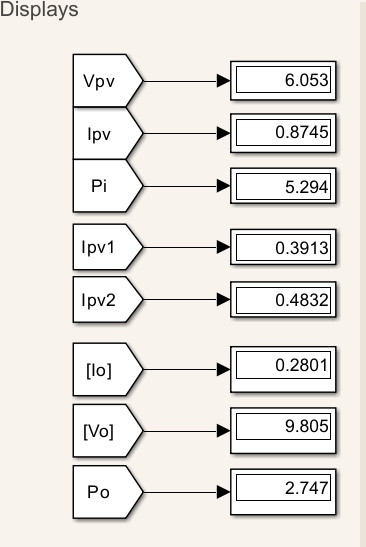
\includegraphics[width=0.5\textwidth]{Figures/5.5.7.png}
    \caption{Displays of Central Interleaved Boost.}
    \label{fig:displays of central interleaved boost actual ratings}
\end{figure}

\begin{figure}[H]
    \centering
    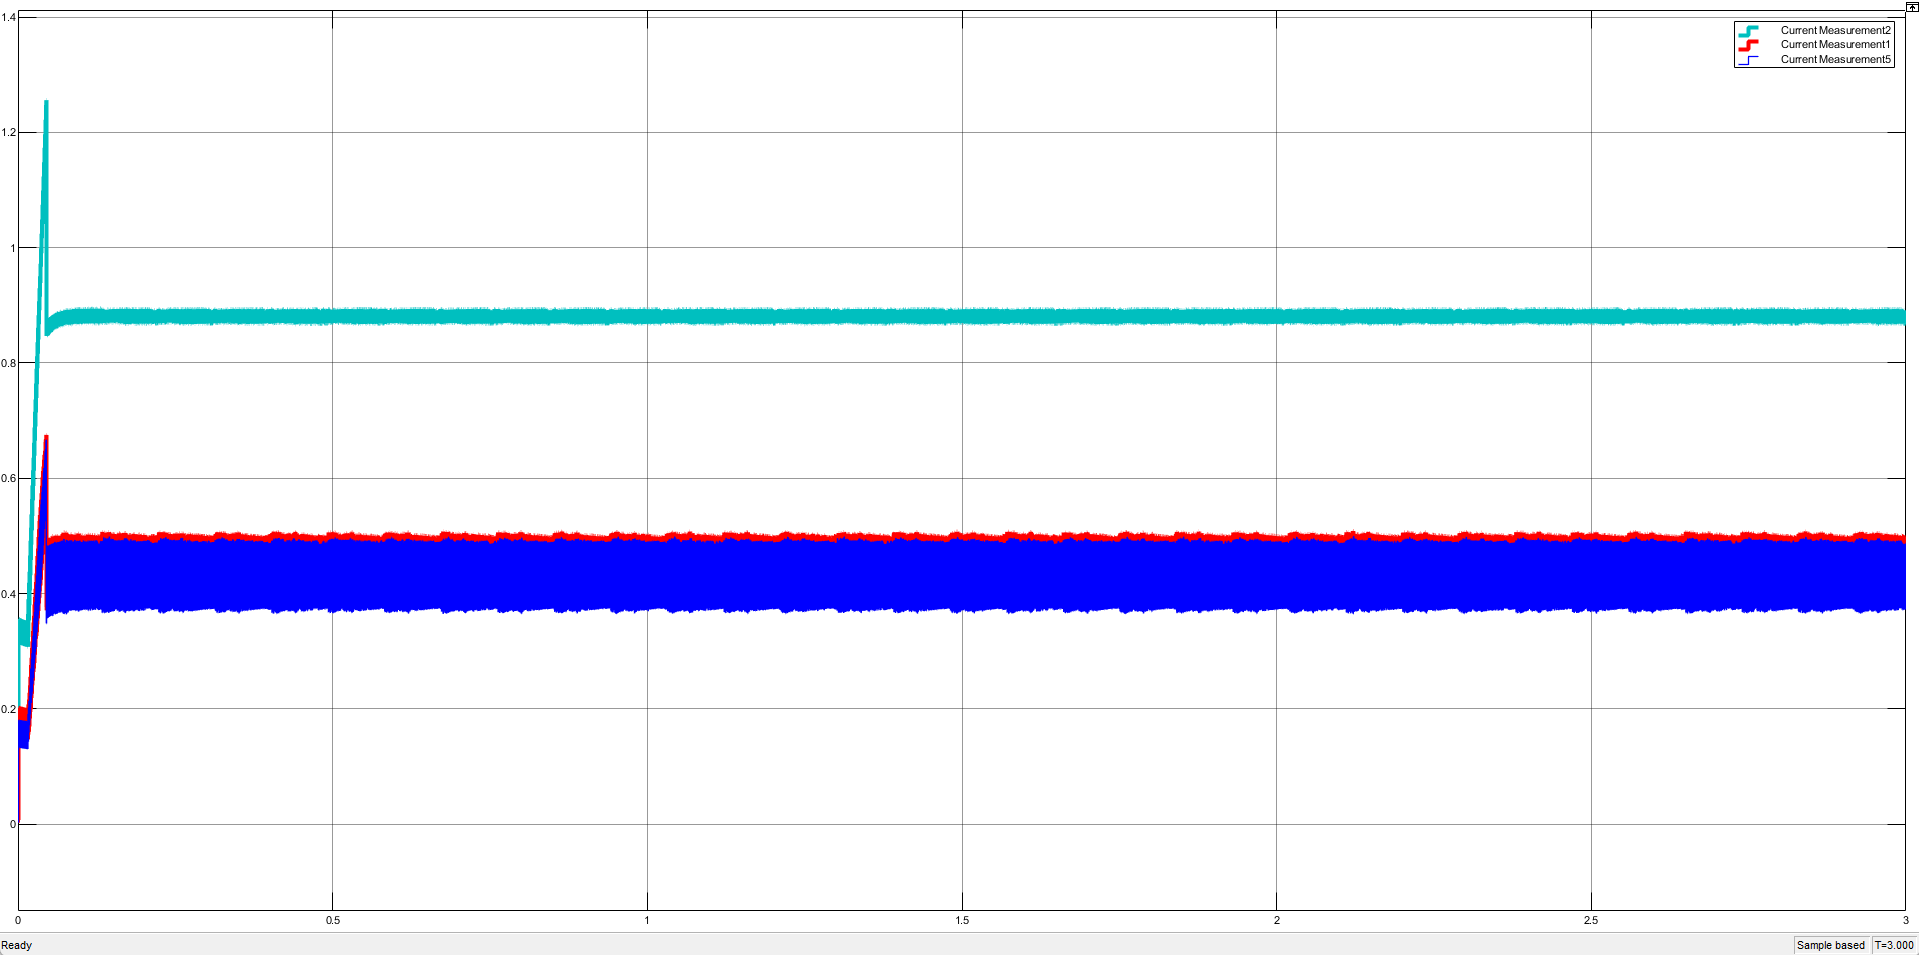
\includegraphics[width=0.9\textwidth]{Figures/5.5.8.png}
    \caption{Total Current, Inductor Current 1, Inductor Current 2.}
    \label{total current , inductor current 1 ,  inductor current 2 of central interleaved boost actual ratings}
\end{figure}

\begin{figure}[H]
    \centering
    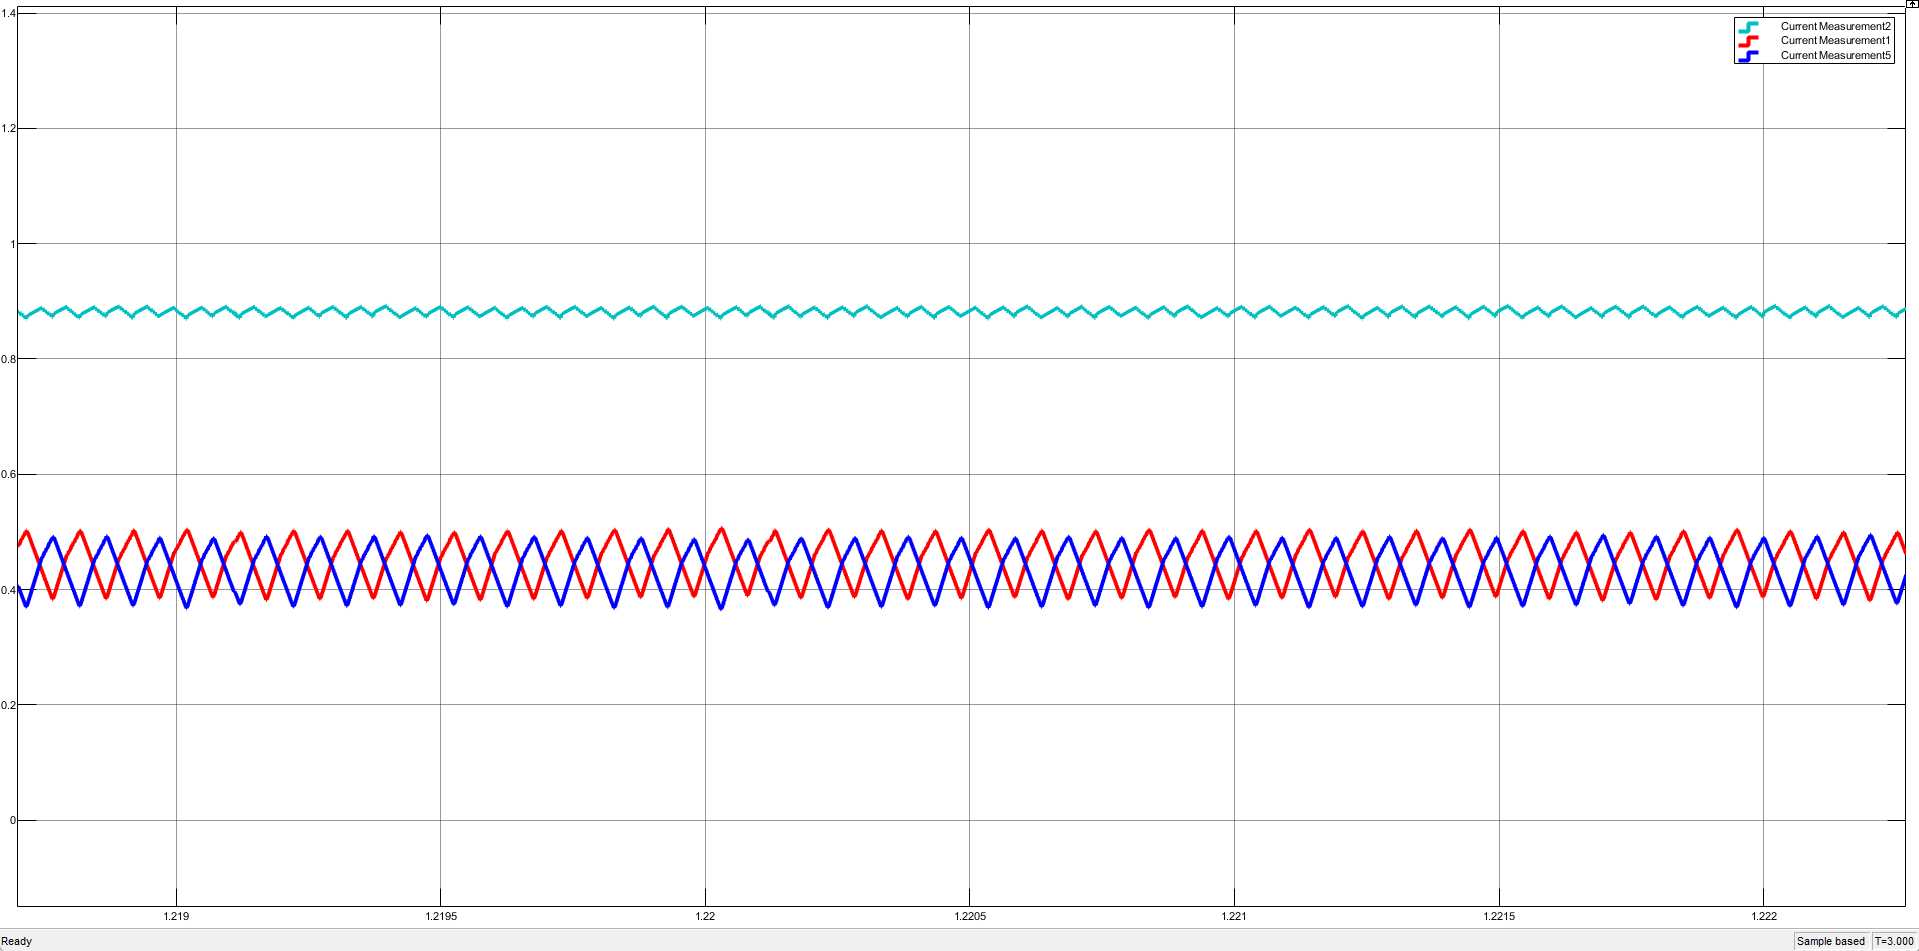
\includegraphics[width=0.9\textwidth]{Figures/5.5.9.png}
    \caption{Total Current, Inductor Current 1, Inductor Current 2.}
    \label{total current , inductor current 1 ,  inductor current 2 zoom of central interleaved boost actual ratings}
\end{figure}

\begin{figure}[H]
    \centering
    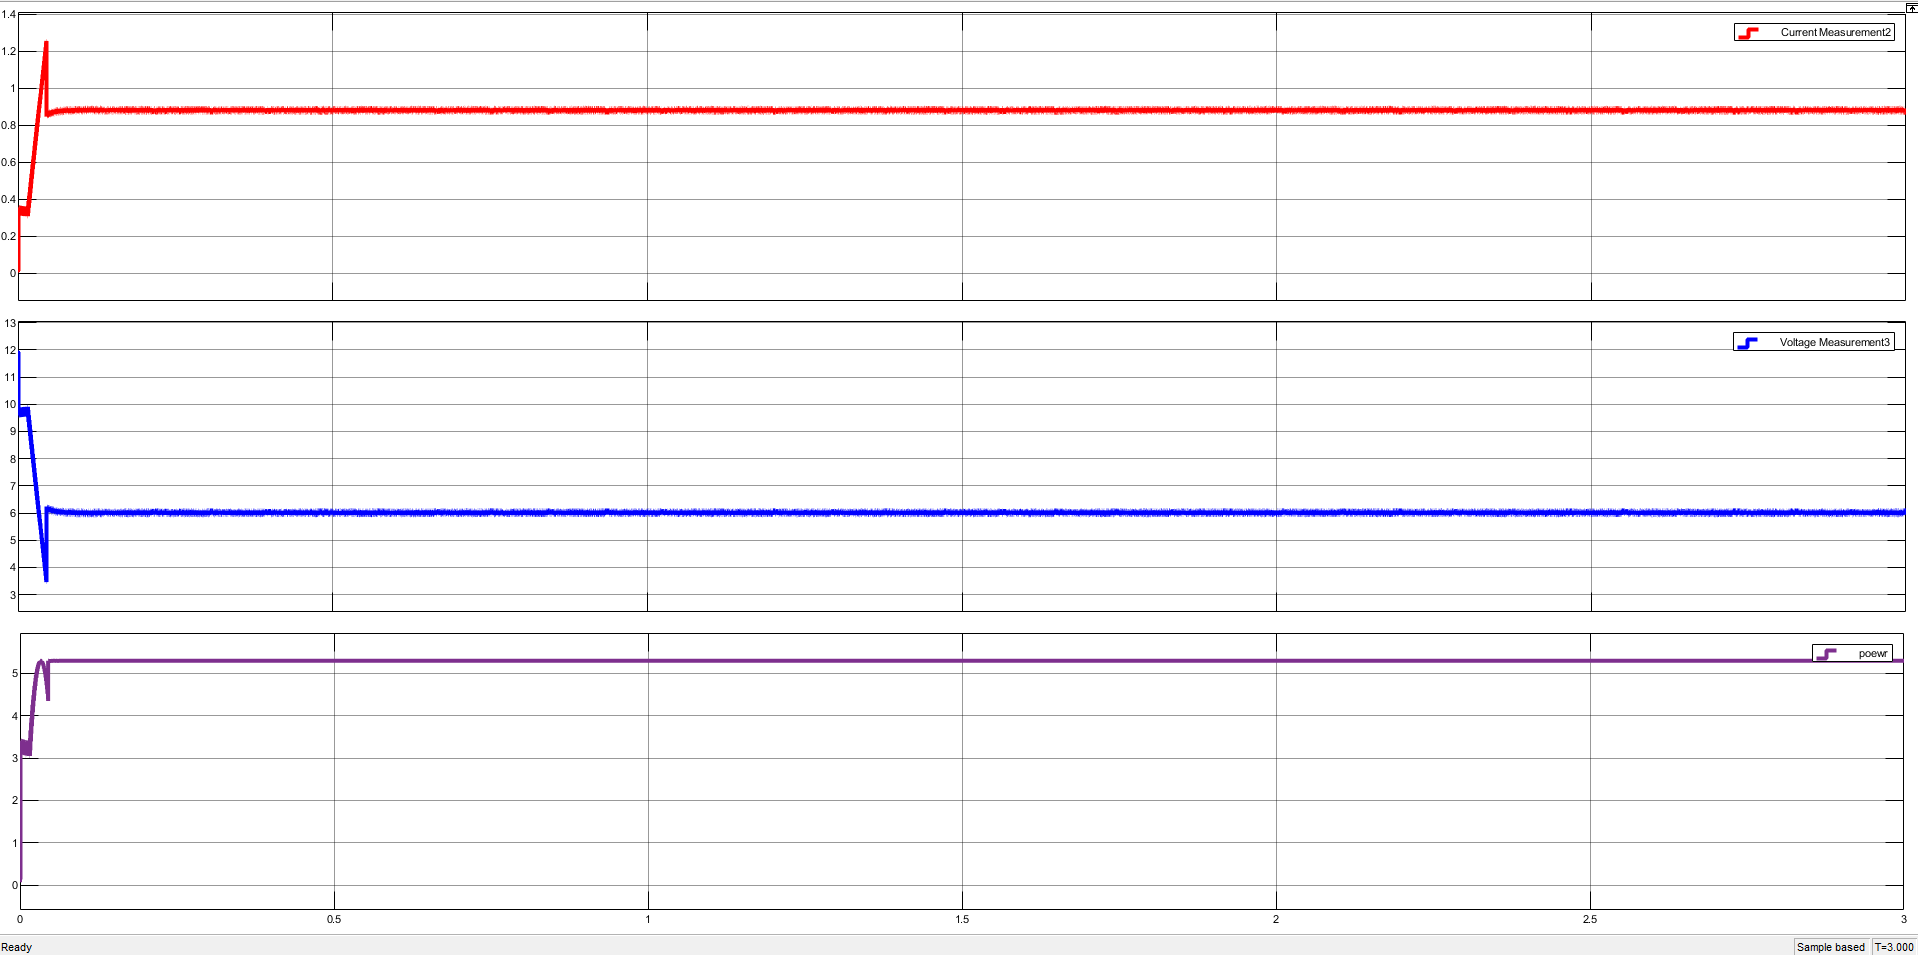
\includegraphics[width=0.9\textwidth]{Figures/5.5.10.png}
    \caption{Input Current, Voltage, Power.}
    \label{input current , voltage , power of central interleaved boost actual ratings}
\end{figure}

\begin{figure}[H]
    \centering
    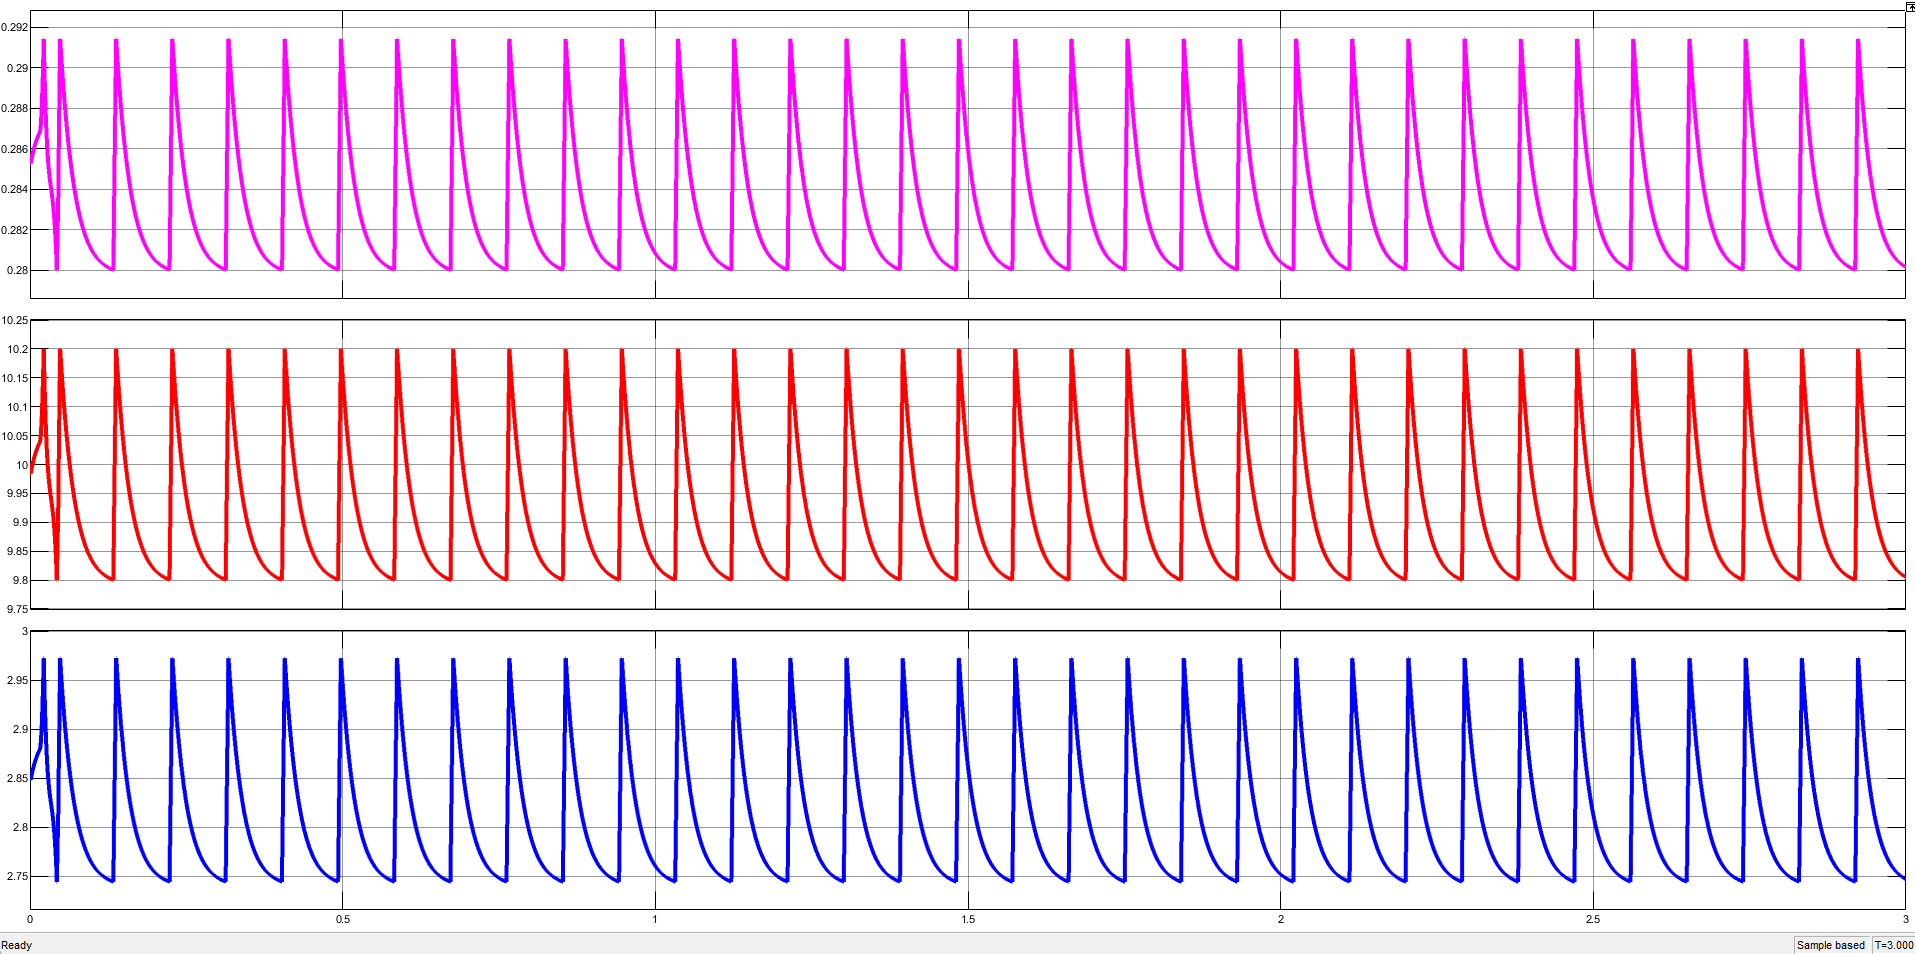
\includegraphics[width=0.9\textwidth]{Figures/5.5.11.png}
    \caption{Output Current, Voltage, Power.}
    \label{output current , voltage , power of central interleaved boost actual ratings}
\end{figure}